\documentclass[11pt,a4paper]{article}

\usepackage[spanish,es-nodecimaldot]{babel}
\usepackage[T1]{fontenc}
\usepackage[utf8]{inputenc}
\usepackage{lmodern}
\usepackage{geometry}
\usepackage{graphicx}
\usepackage{float}
\usepackage{hyperref}
\usepackage{enumitem}
\usepackage{longtable}
\usepackage{array}

\geometry{margin=2.5cm}
\hypersetup{colorlinks=true,linkcolor=black,urlcolor=blue}
\graphicspath{{evidence/screenshots/}}
\setlength{\emergencystretch}{2em}

\title{Asegurar el acceso SSH con autenticación de dos factores y Fail2ban}
\author{Javier Siñuka}
\date{13 de octubre de 2026}

\begin{document}
\maketitle

\section{Resumen y objetivos}
Se realizó un laboratorio de control de acceso SSH, autenticación mediante
clave pública y TOTP, y bloqueo temporal con Fail2ban. Se trabajó sobre un
\textbf{clon aislado} de una máquina virtual Ubuntu; no se modificaron las
políticas de ingreso del host. El objetivo fue ejecutar los pasos de las dos
guías suministradas~\cite{guia-ssh,guia-mfa}, observar tanto éxitos como
rechazos y conservar evidencia auténtica. Se verificó el acceso por clave,
las políticas PAM de denegación y admisión, el segundo factor obligatorio, el
ban de una IP cliente, su regla de firewall y el unban. La matriz completa de
pruebas está en \path{evidence/matrix.csv}.

\section{Introducción y fundamentos}
SSH establece un canal cifrado tras negociar algoritmos y autenticar al
servidor. En la autenticación por clave pública, el cliente prueba la posesión
de su clave privada mediante una firma; la clave pública autorizada se almacena
en el servidor. La frase de paso cifra la clave privada \emph{en el cliente} y
no reemplaza la contraseña de la cuenta remota. \texttt{ssh-agent} conserva
la clave desbloqueada en memoria para evitar repetir la frase de paso en cada
conexión. La clave privada usada en esta práctica se creó exclusivamente para
el laboratorio, con frase de paso, y permaneció fuera de esta carpeta.

Una clave SSH sigue siendo un solo factor de posesión. MFA agrega otra prueba:
con TOTP, un secreto compartido y el tiempo actual producen un código de seis
dígitos que cambia normalmente cada 30 segundos. PAM organiza los módulos de
autenticación y autorización de Linux por servicio. En este caso, OpenSSH usa
PAM para verificar TOTP y, en otra fase separada, para aplicar listas de
usuarios. Fail2ban vigila registros, cuenta fallos por origen y ordena al
firewall bloquear temporalmente una IP. Es una defensa complementaria contra
intentos repetidos y abuso del servicio, con el riesgo de bloquear también a
usuarios legítimos que comparten una IP.

\section{Entorno y metodología}
El host ejecutaba Ubuntu 24.04.5, VirtualBox 7.2.14 y OpenSSH 9.6p1. Se clonó
la VM preexistente \emph{Cybersecurity LabVM Workstation}; el clon
\emph{Crypto SSH 2FA Fail2ban Lab} ejecutó Ubuntu 22.04.1, kernel
5.15.0-60-generic y OpenSSH 8.9p1. Es una distribución derivada de Debian y
permitió usar \texttt{apt}, PAM y los servicios pedidos, sin descargar otra
imagen. Tenía 2 GiB de memoria y dos CPU virtuales. Se instalaron
\texttt{libpam-google-authenticator} 20191231-2 y Fail2ban 0.11.2-6.

La VM recibió \textbf{10.0.2.15/24} en una interfaz NAT. El host se conectó a
\texttt{127.0.0.1:2222}, redirigido al puerto 22 del invitado. El servidor
registró al cliente como \textbf{10.0.2.2}. La consola de VirtualBox quedó
como canal de recuperación independiente de SSH. La figura~\ref{fig:entorno}
muestra dirección y estado de los servicios en esa consola. La captura proviene
de \texttt{VBoxManage controlvm screenshotpng}; se recortó su área vacía solo
al incorporarla al documento.

\begin{figure}[H]
\centering
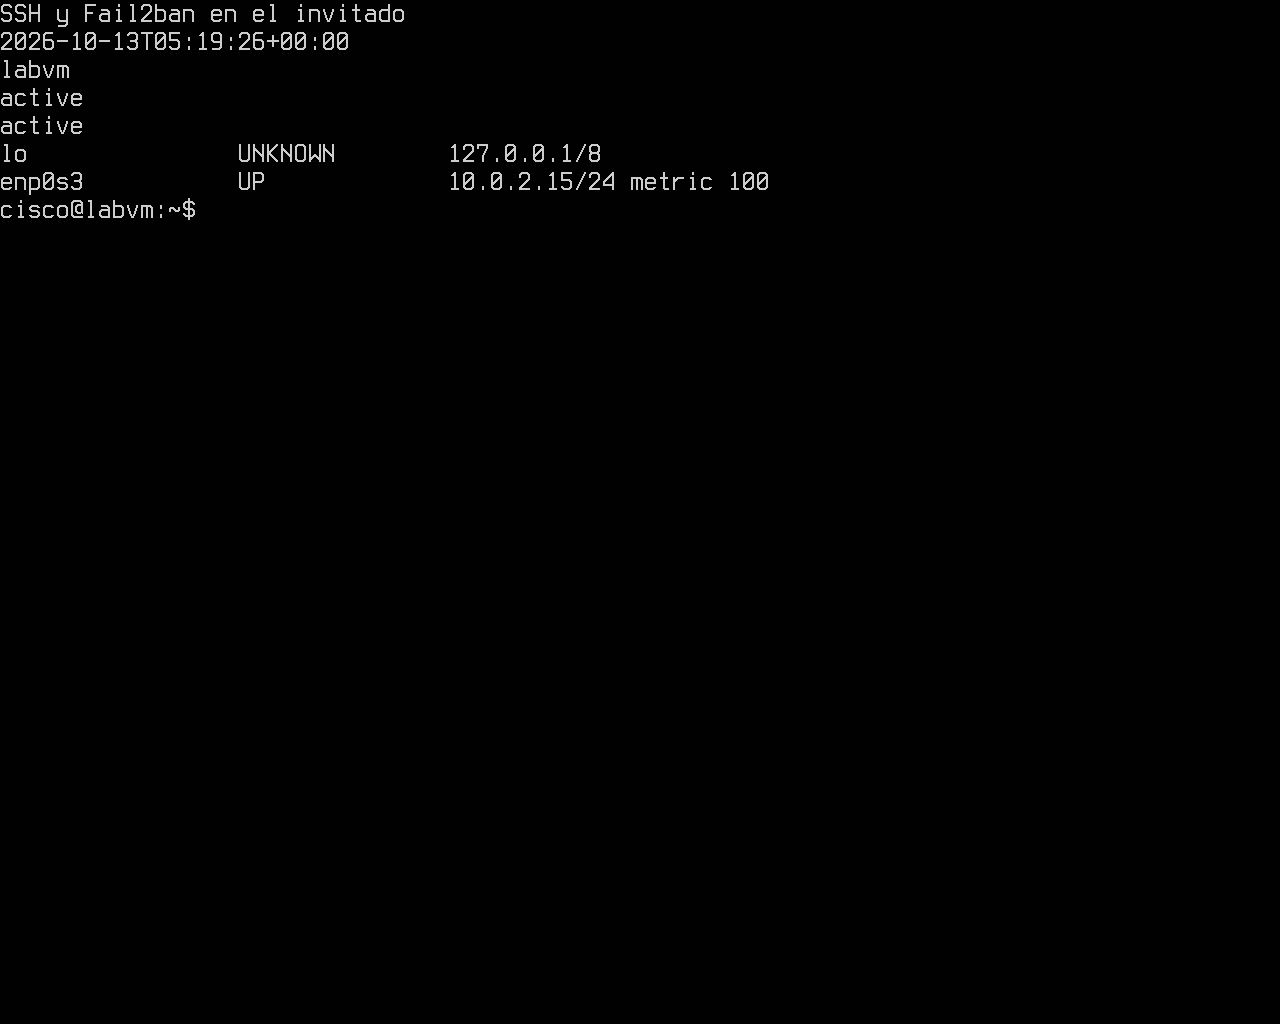
\includegraphics[trim=0 730 0 0,clip,width=\textwidth]{03-guest-baseline.png}
\caption{Consola real del clon: dirección IPv4 y servicios SSH y Fail2ban activos.}
\label{fig:entorno}
\end{figure}

Se tomaron los snapshots \texttt{pre-lab}, \texttt{pre-ssh-auth-change},
\texttt{pre-pam-access-control} y \texttt{pre-mfa-offline}. Un intento de
snapshot en vivo previo a MFA avanzó demasiado lentamente; se canceló, se
apagó el clon limpiamente y se obtuvo el snapshot \texttt{pre-mfa-offline}.
Antes de editar SSH/PAM se copiaron \path{/etc/ssh/sshd_config} y
\path{/etc/pam.d/sshd} a \path{/root/ssh2fa-backup-2026-10-13/}. Antes de
cada recarga se ejecutó \texttt{sshd -t}, se inspeccionaron ajustes efectivos
con \texttt{sshd -T} y se abrió una segunda conexión de prueba.

Las transcripciones en \path{evidence/logs/} registran comandos y resultados
reales. No se incluyeron contraseñas, la clave privada, el secreto TOTP, QR,
OTP vigentes ni códigos de recuperación. Se descartó una captura inicial de
la pantalla de bienvenida porque contenía credenciales de ejemplo.

\section{Desarrollo: control de acceso SSH}
\subsection{Clave pública, usuario normal y root}
Al inicio, \texttt{cisco} ingresó con contraseña (salida 0). La salida de
\texttt{sshd -T} indicó que se admitía contraseña, que la autenticación
interactiva estaba desactivada y que regía
\texttt{PermitRootLogin without-password}. Esta última opción permite
potencialmente root por clave autorizada, pero impide su ingreso por
contraseña. En nuestro ensayo, root no tenía la clave de laboratorio
registrada y su intento terminó con \texttt{Permission denied (publickey)};
esto \emph{no} prueba que todo ingreso root por clave estuviera prohibido.
También se comprobaron las otras cuentas normales presentes en el clon:
\texttt{analyst} y \texttt{sec\_admin} podían usarse localmente, pero SSH las
rechazó con la clave de prueba porque no estaba autorizada para ellas.

Se generó una clave Ed25519 exclusiva y se instaló únicamente el archivo
\texttt{.pub} mediante \texttt{ssh-copy-id -i}. La clave privada quedó con modo
\texttt{0600}, la pública con \texttt{0644} y \texttt{ssh-agent -l} mostró su
huella SHA256. Con \texttt{-i} y \texttt{IdentitiesOnly=yes}, el servidor
aceptó la clave y la sesión devolvió \texttt{cisco}; otra clave fue rechazada.
Recién después se instaló una configuración con
\texttt{PasswordAuthentication no}. La clave continuó funcionando y un
cliente configurado para usar solo contraseña recibió
\texttt{Permission denied (publickey)}. Es importante distinguir
\path{/etc/ssh/ssh_config} y \path{~/.ssh/config}, que configuran al
\emph{cliente}, de \path{/etc/ssh/sshd_config}, que configura al
\emph{servidor}. El cliente toma primero las opciones de línea de comandos,
luego las de usuario y finalmente las globales~\cite{openssh-man}.

\subsection{Algoritmos y vigencia de RSA}
El cliente instalado enumeró Ed25519, ECDSA, RSA y tipos con dispositivo de
seguridad mediante \texttt{ssh -Q key}; esa orden lista capacidades, no
necesariamente los algoritmos habilitados por defecto. La enumeración de
firmas incluyó \texttt{rsa-sha2-256} y \texttt{rsa-sha2-512}. RSA sigue siendo
utilizable con esas firmas SHA-2, especialmente por compatibilidad. La firma
histórica \texttt{ssh-rsa} usa SHA-1 y OpenSSH la deshabilitó por defecto a
partir de 8.8; ello no equivale a retirar las claves RSA~\cite{openssh-rsa}.
Para nuevas claves de este laboratorio se eligió Ed25519. La salida exacta
del cliente figura en \path{evidence/logs/26-host-ssh-algorithms.txt}.

\subsection{\texttt{nonpriv}, claves centrales y banner}
Se creó \texttt{nonpriv} con contraseña local aleatoria no registrada.
\texttt{su - nonpriv -c 'id -un'} funcionó, pero SSH rechazó inicialmente a la
cuenta porque no tenía una clave autorizada. Se configuró
\begin{verbatim}
AuthorizedKeysFile /etc/ssh/authorized-keys/%u .ssh/authorized_keys
\end{verbatim}
y se instaló su clave pública en \path{/etc/ssh/authorized-keys/nonpriv},
con directorio \texttt{root:root 0755} y archivo \texttt{root:root 0644}. Luego
\texttt{nonpriv} ingresó por SSH. La ruta central facilita la auditoría y el
retiro de claves por un administrador, a costa de gestionar permisos y altas
de forma centralizada. \texttt{AuthorizedKeysCommand} y
\texttt{AuthorizedKeysCommandUser} permiten consultar claves desde un
programa y una identidad restringida; requieren controlar ese programa, su
origen de datos y los registros de auditoría. No se conectó LDAP en esta
práctica~\cite{openssh-man}.

Se agregó un banner académico en \path{/etc/ssh/ssh2fa-banner} y la directiva
\texttt{Banner} en \path{/etc/ssh/sshd_config.d/30-banner.conf}. El cliente
mostró el texto antes de completar la autenticación. La ruta
\path{/etc/sshd_config} mencionada en la guía no era la del servidor instalado.

\subsection{Listas de acceso PAM}
Se probaron dos estados distintos de \path{/etc/pam.d/sshd}. Primero, una regla
\texttt{account required pam\_listfile.so} con \texttt{sense=deny} rechazó a
\texttt{nonpriv} y dejó entrar a \texttt{cisco}. Después, al sustituirla por
\texttt{sense=allow} y listar solamente \texttt{cisco}, este entró y
\texttt{nonpriv} fue rechazado. Los rechazos quedaron registrados como
\texttt{pam\_listfile(sshd:account): Refused user nonpriv}. Se usó la fase
\texttt{account} para que la comprobación también ocurriera tras una clave
pública válida. Se eligió \texttt{onerr=fail} para evitar permitir el ingreso
si falta el archivo de política. Cada lista tuvo dueño root y modo
\texttt{0600}. Antes de MFA, se restauró el PAM original para no mezclar
políticas y confundir la causa de cada resultado.

\section{Desarrollo: autenticación de dos factores}
Como \texttt{cisco}, se ejecutó \texttt{google-authenticator} en modo TOTP,
con prohibición de reutilizar códigos, ventana de tres pasos temporales y
límite de tres intentos cada 30 segundos. El archivo
\path{~/.google_authenticator} quedó propiedad del usuario y modo
\texttt{0400}. Los códigos de recuperación quedaron dentro de ese archivo;
no se imprimieron ni copiaron al repositorio. Una instalación real debe
custodiarlos de forma separada y segura.

Se respaldaron de nuevo PAM y la configuración de SSH. La fase probada usó
\begin{verbatim}
PubkeyAuthentication yes
PasswordAuthentication no
KbdInteractiveAuthentication yes
UsePAM yes
AuthenticationMethods publickey,keyboard-interactive
\end{verbatim}
En PAM se comentó \texttt{@include common-auth} para no pedir además la
contraseña local y se agregó
\texttt{auth required pam\_google\_authenticator.so}. No se usó
\texttt{nullok}; el usuario protegido no podía omitir TOTP. La
figura~\ref{fig:mfa-config} muestra los archivos reales. Configurar solo
\texttt{PasswordAuthentication no} no habría bastado para desactivar otros
métodos interactivos. \texttt{AuthenticationMethods} exige ambas etapas en
el orden indicado~\cite{openssh-man}.

\begin{figure}[H]
\centering
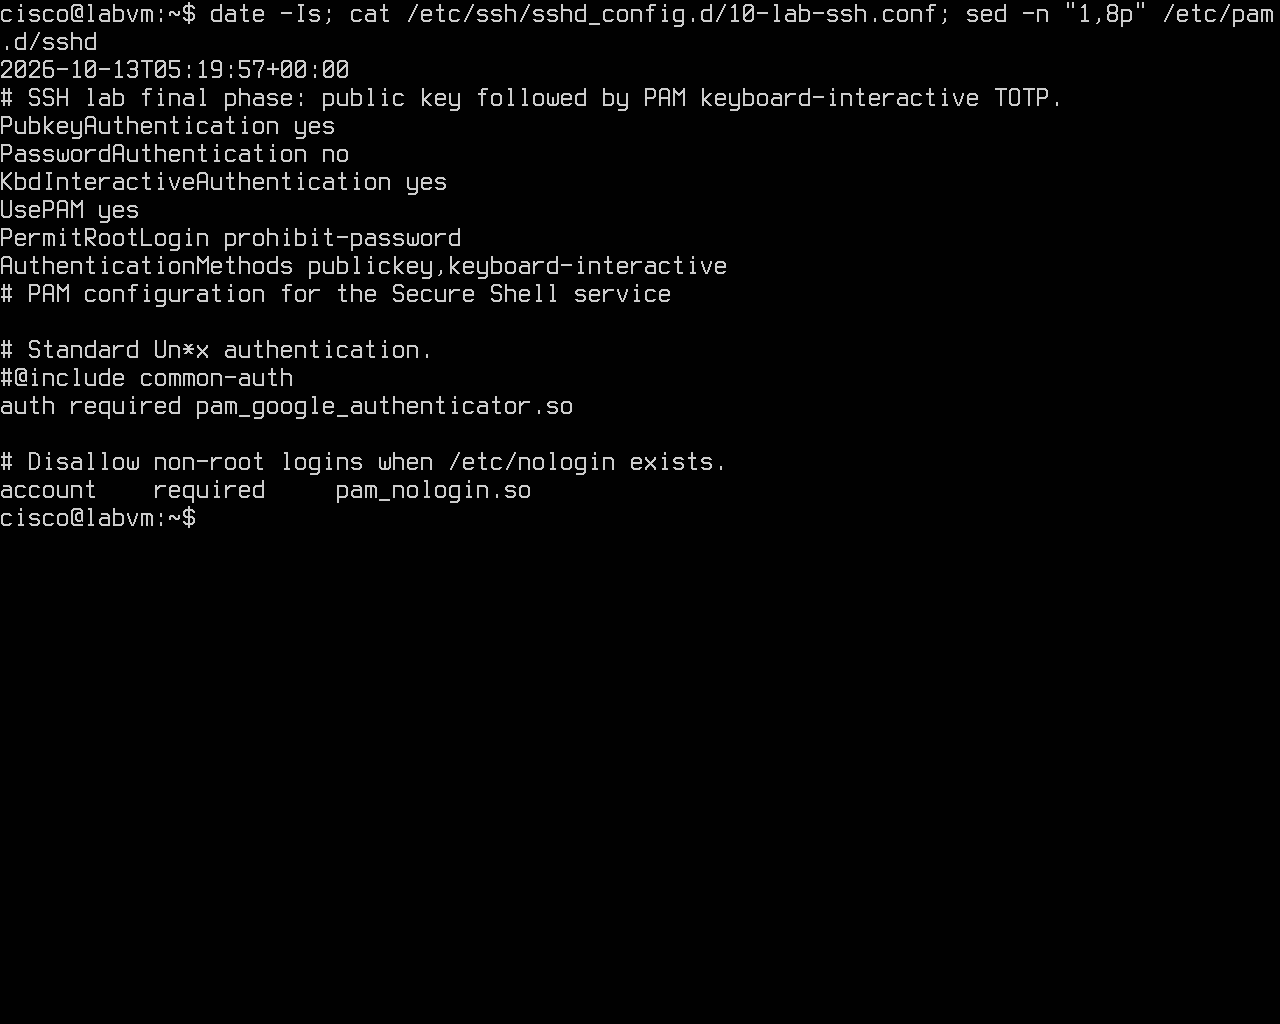
\includegraphics[trim=0 420 0 0,clip,width=\textwidth]{04-mfa-configuration.png}
\caption{Configuración efectiva de la fase MFA: clave pública seguida de PAM/TOTP.}
\label{fig:mfa-config}
\end{figure}

No hubo un teléfono enrolado. Para comprobar el paso criptográfico se usó
\path{scripts/totp_local_client.py} \textbf{dentro de la VM}: lee el secreto
localmente, calcula HMAC-SHA1/TOTP y entrega el código a una segunda sesión
SSH, sin imprimirlo. Es una emulación de laboratorio y no demuestra separación
física de dispositivos. Una clave válida más un código actual abrió la sesión
(salida 0 y marcador de comando observado), como muestra la
figura~\ref{fig:mfa-ok}. Un código incorrecto y uno vencido terminaron con
salida 255; una clave incorrecta fue rechazada antes del prompt TOTP. Desde el
host, la clave correcta sin código fue aceptada en la primera etapa, pero SSH
continuó solicitando \texttt{keyboard-interactive} y denegó la sesión. El
registro del servidor mostró \texttt{Accepted google\_authenticator} para
los éxitos y \texttt{Invalid verification code} para los fallos.

\begin{figure}[H]
\centering
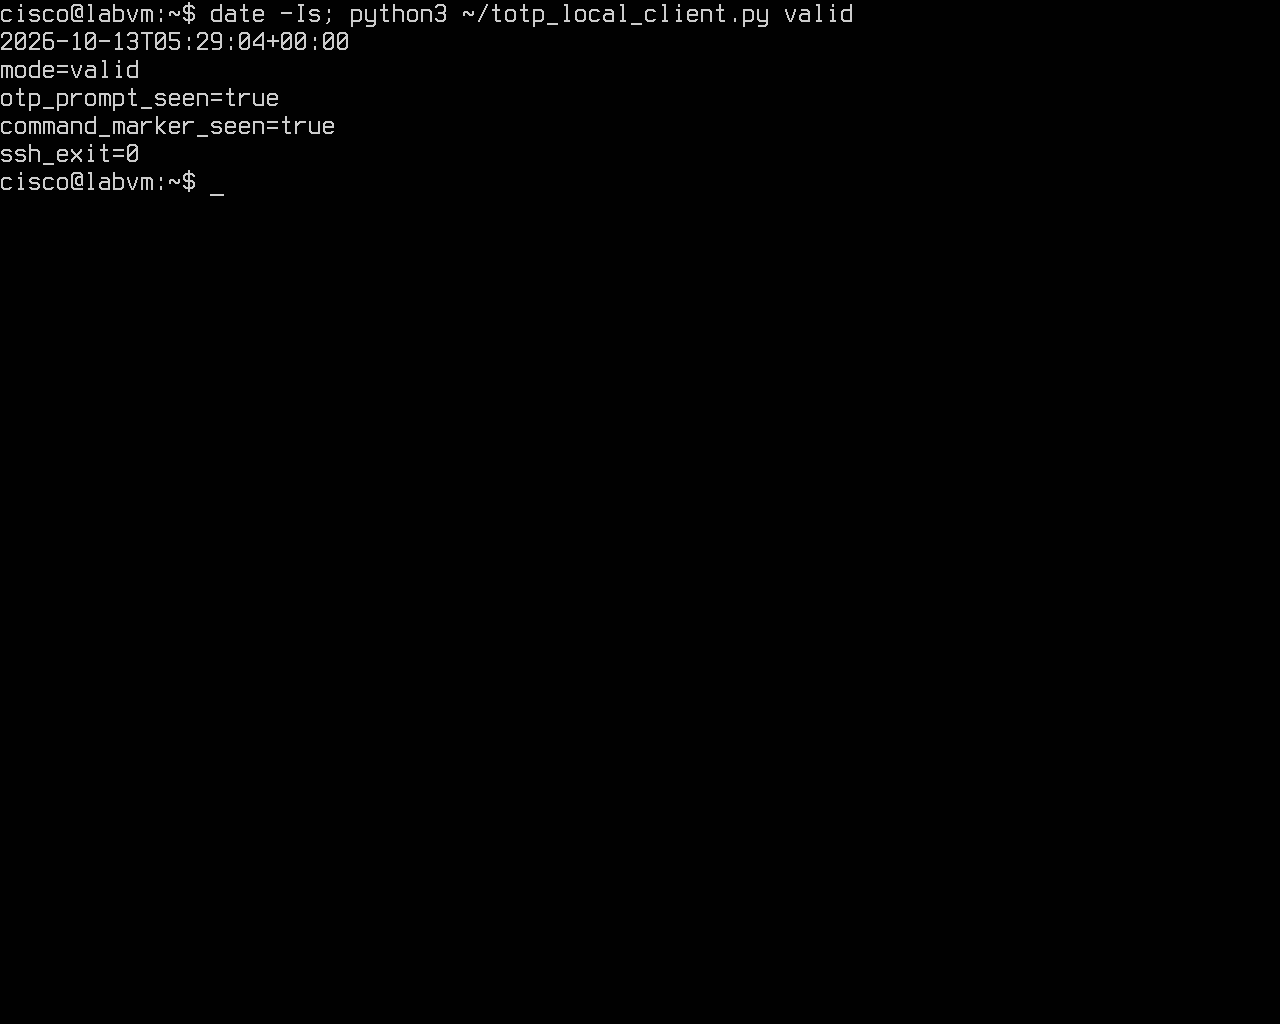
\includegraphics[trim=0 760 0 0,clip,width=\textwidth]{05-mfa-success.png}
\caption{Sesión SSH local de prueba completada con clave y TOTP actual; el código no se muestra.}
\label{fig:mfa-ok}
\end{figure}

\begin{figure}[H]
\centering
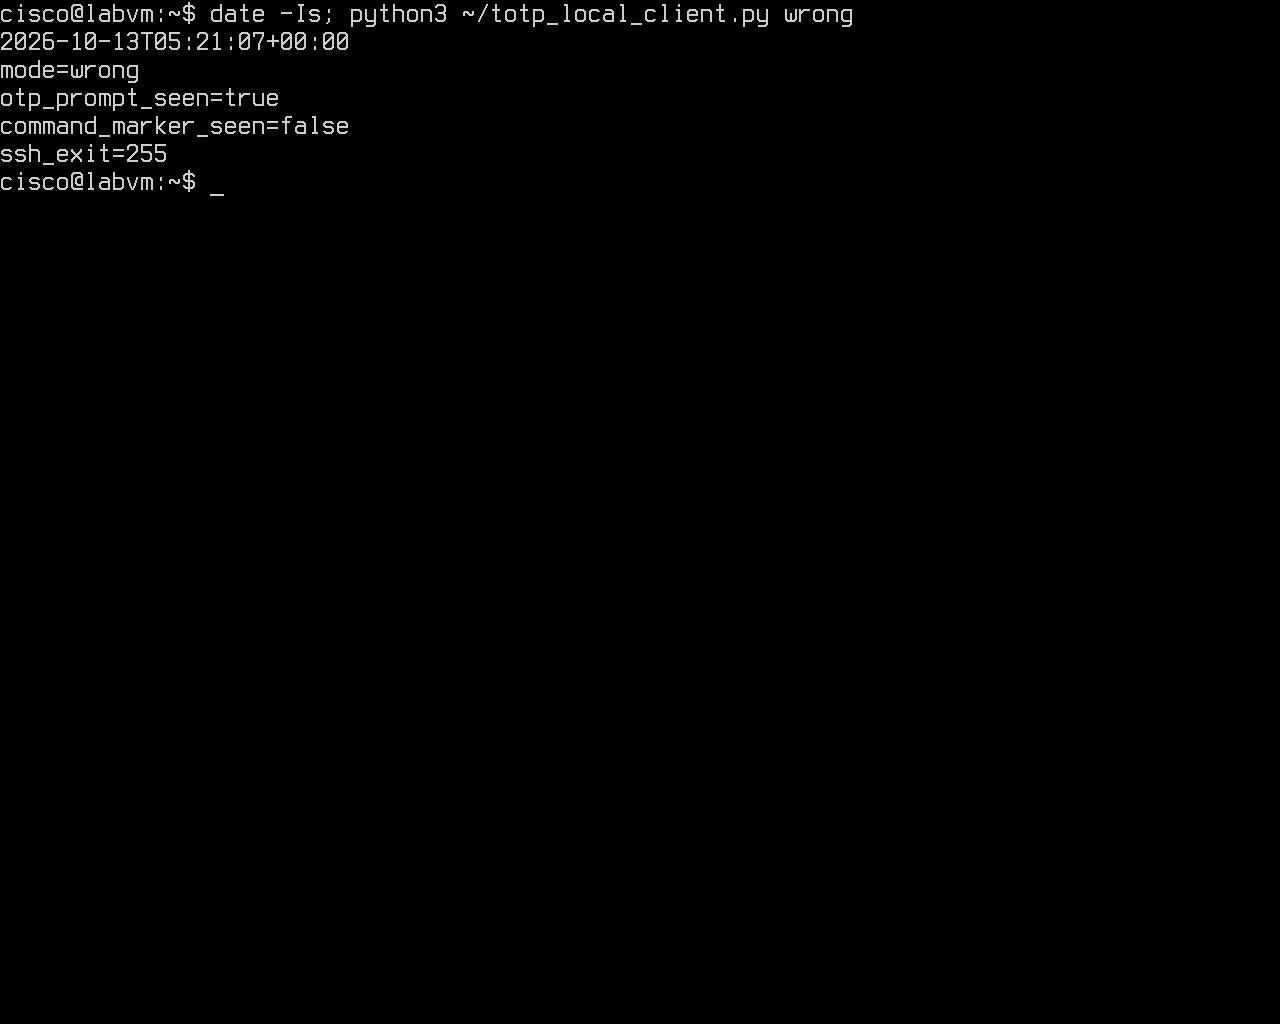
\includegraphics[trim=0 760 0 0,clip,width=\textwidth]{06-mfa-wrong-code.png}
\caption{Código TOTP incorrecto: se solicita el segundo factor, pero no se ejecuta el comando remoto.}
\end{figure}

Si se pierde el dispositivo, la consola de VirtualBox y un snapshot permiten
recuperar el clon sin cambiar la política del host. En producción deben
custodiarse códigos de recuperación de un solo uso y re-enrolar de forma
controlada si se pierde el secreto. \texttt{nullok} permite transiciones o
excepciones por cuenta, pero deja a esas cuentas con un solo factor; no se
aplicó aquí. El archivo por usuario puede controlar reutilización, ventana
temporal, límite de intentos y códigos de emergencia; ampliar la ventana o
permitir reutilización reduce la resistencia ante códigos capturados. La
salida real de \texttt{google-authenticator --help} mostró las opciones
\texttt{-d}, \texttt{-w}, \texttt{-r}, \texttt{-R}, \texttt{-e} y
\texttt{-C} para una inscripción automatizada. La guía también propone un
tercer factor: reactivar \texttt{common-auth} haría que PAM pidiese
contraseña local además de TOTP después de la clave SSH. Estas variantes se
explican, pero no se activaron ni se presentan como resultados experimentales.

\section{Desarrollo: Fail2ban}
Se instaló Fail2ban y se configuró un jail \texttt{[sshd]} en
\path{/etc/fail2ban/jail.d/sshd.local} con
\texttt{enabled=true}, \texttt{bantime=10m}, \texttt{findtime=10m} y
\texttt{maxretry=5}. La opción correcta es \texttt{enabled}, no
\texttt{enable} como aparece en la guía. En esta VM existía
\path{/var/log/auth.log} y \texttt{rsyslog} estaba activo; se eligió
\texttt{backend=polling}. El firewall usó \texttt{iptables-multiport} sobre
\texttt{iptables v1.8.7 (nf\_tables)}. Después de un breve inicio del
servicio, \texttt{fail2ban-client status sshd} mostró el archivo vigilado y
ninguna IP baneada.

Se generaron fallos controlados exclusivamente contra el clon desde el host.
Al arrancar el jail se habían registrado tres fallos MFA recientes desde
\texttt{10.0.2.2}; Fail2ban también los detectó. Dos intentos de usuario
inválido posteriores completaron el umbral de cinco dentro de diez minutos;
un sexto evento se registró prácticamente a la vez que el ban. El registro
mostró \texttt{Ban 10.0.2.2}. \texttt{iptables -L} confirmó el salto de
\texttt{INPUT} a \texttt{f2b-sshd} para el puerto 22 y una regla
\texttt{REJECT} para esa IP. Un cliente autorizado desde el host quedó
bloqueado antes del banner y agotó el tiempo de espera. El segundo ban
controlado permitió capturar en pantalla la regla activa de la
figura~\ref{fig:ban}.

\begin{figure}[H]
\centering
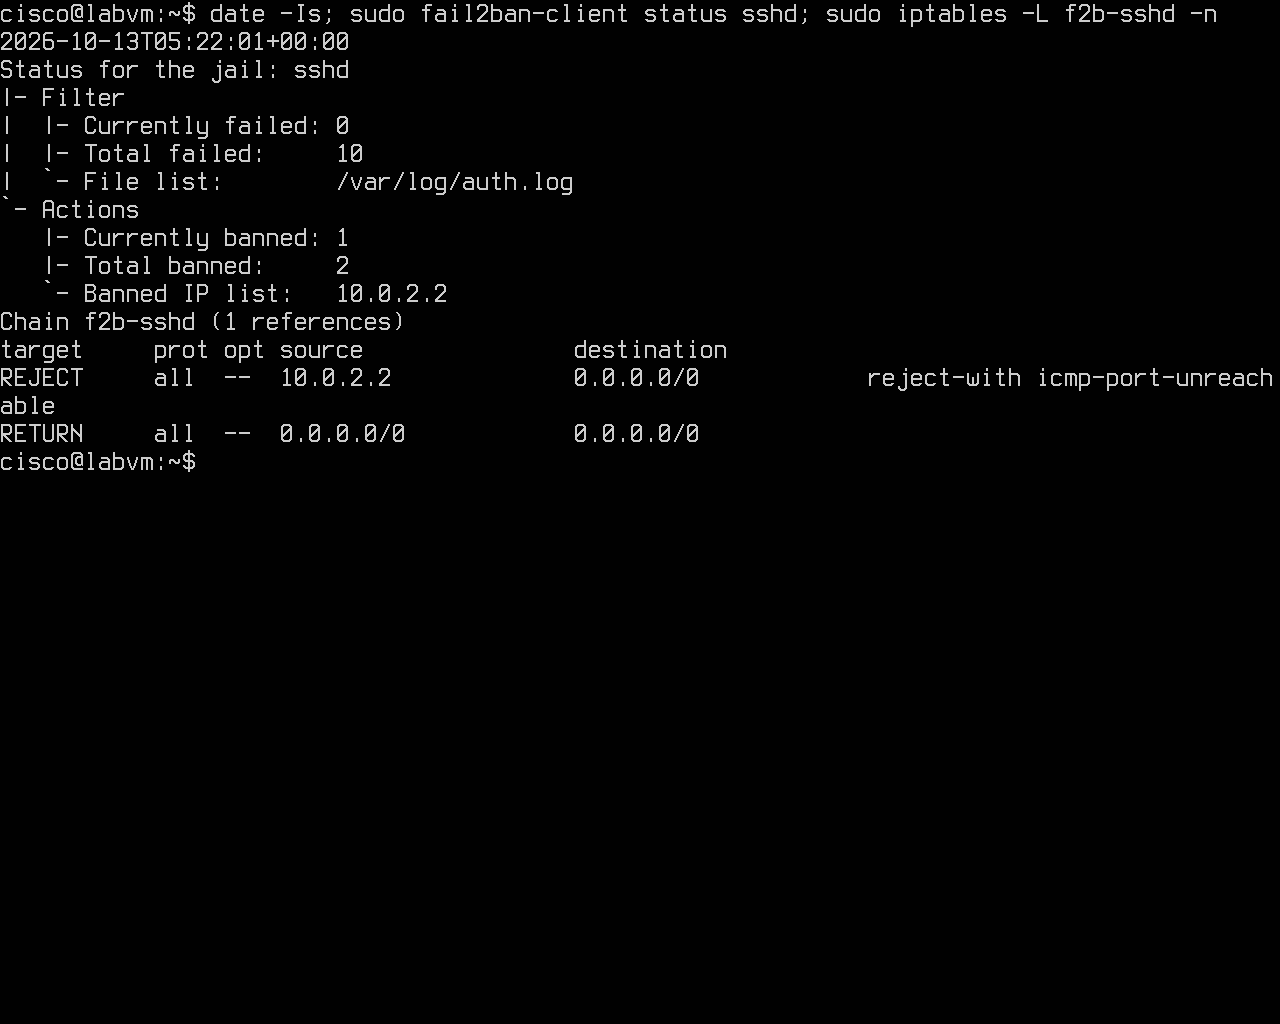
\includegraphics[trim=0 560 0 0,clip,width=\textwidth]{07-fail2ban-ban-firewall.png}
\caption{Fail2ban registra la IP baneada y \texttt{iptables} contiene la regla de rechazo.}
\label{fig:ban}
\end{figure}

Desde la consola se ejecutó \texttt{fail2ban-client set sshd unbanip
10.0.2.2}. El jail pasó a cero IP baneadas y la regla \texttt{REJECT}
desapareció (figura~\ref{fig:unban}). Tras el unban, el host volvió a
alcanzar la etapa TOTP: el servidor aceptó la clave y ofreció
\texttt{keyboard-interactive}. No se completó un ingreso desde el host porque
el secreto TOTP permaneció dentro del clon. El cliente local sí completó de
nuevo MFA. Esto distingue recuperación de red desde la IP antes baneada de
una autenticación completa desde ese cliente.

\begin{figure}[H]
\centering
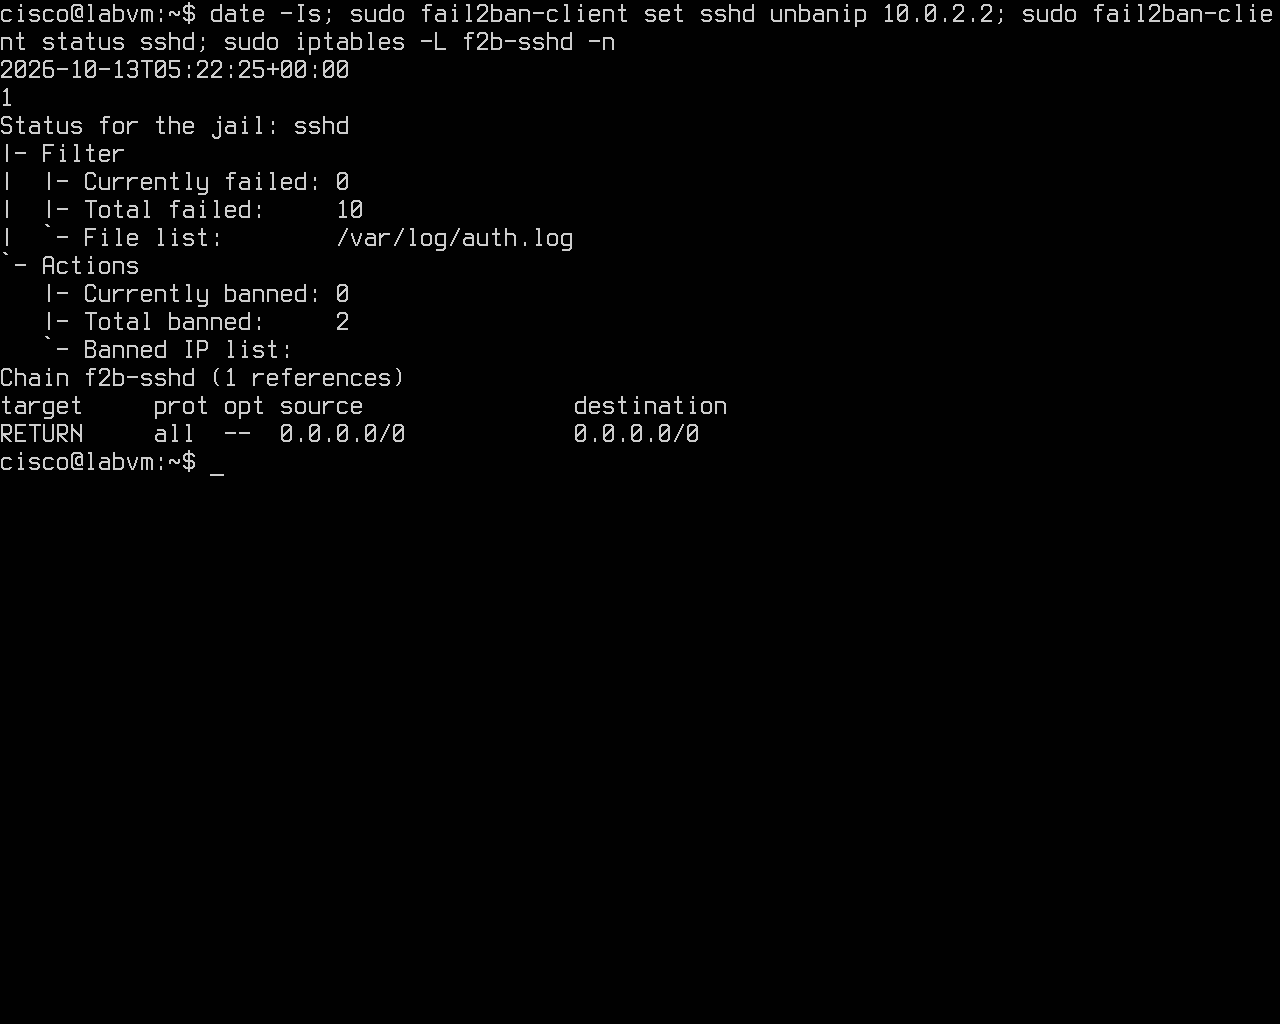
\includegraphics[trim=0 500 0 0,clip,width=\textwidth]{08-fail2ban-unban.png}
\caption{Desbloqueo manual: lista vacía de IP baneadas y ausencia de la regla \texttt{REJECT}.}
\label{fig:unban}
\end{figure}

Fail2ban también puede vigilar otros servicios con filtros adecuados, por
ejemplo servidores web, correo y servicios de archivos; sus acciones pueden
enviar avisos por correo además de modificar el firewall~\cite{fail2ban-doc}.
Depende de registros correctos y de una acción de firewall efectiva. Un ban
por IP puede afectar a usuarios legítimos detrás del mismo NAT y es menos
eficaz ante ataques distribuidos. En este ensayo, la consola de VirtualBox
permitió desbanear sin depender de la IP bloqueada.

\section{Resultados y análisis}
La tabla~\ref{tab:matriz} resume los resultados observados. \emph{Pasa}
indica que el comportamiento coincidió con lo esperado; \emph{parcial}
explicita el límite de la prueba desde el host. El CSV adjunto incluye
procedimiento, fase de configuración, origen y archivo de evidencia por fila.

\footnotesize
\setlength{\tabcolsep}{3pt}
\begin{longtable}{>{\raggedright\arraybackslash}p{0.07\textwidth}>{\raggedright\arraybackslash}p{0.36\textwidth}>{\raggedright\arraybackslash}p{0.17\textwidth}>{\raggedright\arraybackslash}p{0.28\textwidth}}
\caption{Matriz resumida de pruebas ejecutadas.}\label{tab:matriz}\\
\hline
ID & Escenario & Esperado & Observado \\
\hline
\endfirsthead
\hline
ID & Escenario & Esperado & Observado \\
\hline
\endhead
T01 & VM alcanzable y SSH activo & Servicio activo & \texttt{10.0.2.15}; activo \\
T02 & Usuario normal antes de claves & Ingreso con contraseña & \texttt{cisco}; salida 0 \\
T03 & Root con clave no autorizada & Rechazo & Salida 255; clave ausente \\
T04 & Clave pública autorizada & Ingreso & \texttt{cisco}; salida 0 \\
T05 & Clave equivocada & Rechazo & \texttt{Permission denied} \\
T06 & Solo contraseña tras desactivarla & Rechazo & Salida 255; clave sigue válida \\
T07 & \texttt{nonpriv} antes de clave & Local sí; SSH no & \texttt{su} sí; SSH salida 255 \\
T08 & \texttt{nonpriv} con clave central & Ingreso SSH & \texttt{nonpriv}; salida 0 \\
T09 & Banner SSH & Visible antes de ingreso & Texto ASCII observado \\
T10 & PAM denylist & Rechazar listado & \texttt{nonpriv} no; \texttt{cisco} sí \\
T11 & PAM allowlist & Admitir listado & \texttt{cisco} sí; \texttt{nonpriv} no \\
T12 & Clave y TOTP actual & Ingreso & Marcador y salida 0 \\
T13 & Clave válida sin TOTP & Rechazo & Pide segundo factor; salida 255 \\
T14 & TOTP incorrecto y vencido & Rechazo & Ambos salida 255 \\
T15 & Clave errónea durante MFA & Rechazo previo a TOTP & Sin prompt; salida 255 \\
T16 & Jail SSH de Fail2ban & Activo & \texttt{sshd}; \texttt{auth.log} vigilado \\
T17 & Umbral y regla de bloqueo & Ban de IP cliente & \texttt{10.0.2.2}; \texttt{REJECT} \\
T18 & Conexión tras ban & Bloqueo & Timeout antes del banner \\
T19 & Unban y reconexión & Recuperación & Host vuelve a TOTP; MFA local sí (parcial) \\
T20 & Tercer factor opcional & Opcional & No ejecutado \\
\end{longtable}
\setlength{\tabcolsep}{6pt}
\normalsize

El primer \texttt{fail2ban-client status} se lanzó inmediatamente tras iniciar
el servicio y aún no encontró su socket; la siguiente consulta sí devolvió el
jail activo. Los fallos que contaron para el primer ban incluyeron pruebas MFA
previas. En las pruebas TOTP negativas iniciales el cliente de prueba quedó
esperando un segundo prompt; se ajustó
\texttt{NumberOfPasswordPrompts=1} y se repitieron. Los resultados definitivos
son los de \path{evidence/logs/33-mfa-totp-retake.txt}. Estos detalles se
conservan para no presentar una secuencia más limpia que la observada.

\section{Discusión y respuestas a las guías}
La lista de denegación sirve cuando casi todos los usuarios pueden entrar y
solo unos pocos son excepciones. La lista de admisión es más fácil de auditar
cuando solo un grupo reducido debe tener acceso remoto; una cuenta puede
seguir siendo válida en la consola local y ser rechazada por SSH. En ambos
casos se deben gestionar cambios de personal, propiedad de archivos y
recuperación ante errores. La política PAM de tipo \texttt{account} aplicada
aquí se verificó también con claves públicas.

El ensayo de root mostró la diferencia entre la política efectiva y una
prueba concreta: \texttt{without-password} no equivale a
\texttt{PermitRootLogin no}. El usuario \texttt{nonpriv} falló primero porque
no tenía clave autorizada, no por carecer de contraseña local. La ruta central
de claves permitió autorizarlo; en un servicio real habría que revocar claves
obsoletas y registrar cada alta.

Tras los fallos, Fail2ban creó una regla para la IP cliente y bloqueó nuevas
conexiones al puerto SSH. \texttt{iptables -L} exhibió la cadena
\texttt{f2b-sshd} y el \texttt{REJECT}; el unban retiró esa entrada. Otros
filtros pueden vigilar servicios web o de correo. Una acción de aviso por
correo es posible, pero no se configuró ni verificó un envío en esta práctica.
El modo de tercer factor, las excepciones por cuenta y la automatización de
enrolamiento quedaron como opciones explicadas, sin atribuirles pruebas.

\section{Conclusiones}
El laboratorio demostró que se puede exigir una clave SSH y un segundo paso
TOTP, restringir cuentas mediante PAM y bloquear temporalmente la IP de un
cliente que acumula fallos. Las pruebas negativas fueron tan importantes como
las positivas: detectaron el efecto real de cada configuración y permitieron
revertirla antes de la fase siguiente. Los snapshots, las copias de archivos,
la validación con \texttt{sshd -t} y la consola separada evitaron perder el
acceso durante los cambios.

La principal limitación es que el TOTP válido se generó dentro de la VM con un
cliente emulado; se verificó la secuencia criptográfica y de OpenSSH, pero no
la custodia en un teléfono independiente. Después del unban, el host recuperó
conectividad hasta la solicitud del segundo factor, mientras el cliente local
completó MFA. El modo opcional de tres factores y las alertas de Fail2ban no
fueron ejecutados. Las configuraciones y scripts de esta carpeta permiten
repetir el ensayo o restaurar el clon.
Las claves SSH son apropiadas para administrar cuentas remotas, PAM permite
definir quién puede entrar y TOTP agrega protección cuando una clave podría
ser robada. Fail2ban aporta control de frecuencia para un servicio expuesto,
siempre que se vigilen los registros y se conserve una vía de recuperación.

\clearpage
\section{Anexo: archivos y recuperación}
\begin{itemize}[noitemsep]
\item \path{configs/}: directivas SSH, reglas PAM, banner y jail de Fail2ban.
\item \path{scripts/guest-phase.sh}: preparación, fases separadas y rollback
dentro de un invitado de laboratorio.
\item \path{scripts/totp_local_client.py}: cliente TOTP local que no imprime
secretos ni códigos.
\item \path{evidence/matrix.csv}: procedimientos, resultados y nombres de
evidencia. \path{evidence/logs/} contiene transcripciones; las capturas reales
están en \path{evidence/screenshots/}.
\end{itemize}
Para restaurar el clon ejecutado se dispone de la consola y de las copias en
\path{/root/ssh2fa-backup-2026-10-13/}. El procedimiento reproducible y la
invocación de rollback figuran en \path{README.md}. No se debe reutilizar
ninguna credencial de este clon en un sistema de producción.

\begin{thebibliography}{9}
\bibitem{guia-ssh}
Material de la actividad, \emph{Control de acceso en ssh sin todas las vm}.
PDF suministrado en esta carpeta.
\bibitem{guia-mfa}
Material de la actividad, \emph{Copia de Two-factor authentication (2FA)}.
PDF suministrado en esta carpeta.
\bibitem{openssh-rsa}
OpenSSH, \emph{Release Notes}, sección OpenSSH 8.8: transición de firmas
\texttt{ssh-rsa} a RSA/SHA-2.
\url{https://www.openssh.com/releasenotes.html}.
Consulta: 13 de octubre de 2026.
\bibitem{openssh-man}
OpenBSD, \emph{sshd\_config(5)} y \emph{ssh\_config(5)}.
\url{https://man.openbsd.org/sshd_config.5} y
\url{https://man.openbsd.org/ssh_config.5}.
Consulta: 13 de octubre de 2026.
\bibitem{fail2ban-doc}
Fail2ban, \emph{jail.conf} y acciones, repositorio oficial.
\url{https://github.com/fail2ban/fail2ban/blob/master/config/jail.conf}.
Consulta: 13 de octubre de 2026.
\end{thebibliography}
\end{document}
